\documentclass{article}
\usepackage{amsmath}
\usepackage{Sweave}
\begin{document}
\Sconcordance{concordance:chn_binom.tex:chn_binom.Rnw:%
1 2 1 1 0 33 1 1 2 7 0 1 2 1 1 1 2 6 0 1 1 6 0 1 2 9 1 1 2 1 0 3 1 6 0 %
1 2 3 1 1 4 3 0 2 1 1 2 1 0 1 2 1 0 1 2 1 0 1 11 13 0 1 2 2 1 1 2 17 0 %
1 2 38 1 1 2 1 0 1 8 7 0 1 1 4 0 1 2 2 1 1 2 7 0 1 2 3 1 1 2 1 0 1 8 7 %
0 1 1 4 0 1 2 2 1 1 2 7 0 1 2 5 1 1 2 1 0 1 35 33 0 2 1 4 0 1 2 2 1 1 %
39 1 2 2 1 1 43 1 2 3 1 1 4 3 0 2 1 1 2 1 0 1 2 1 0 1 2 1 0 1 11 10 0 1 %
1 1 10 9 0 2 1 20 0 1 2 3 1}


\title{Parameter estimation by maximum likelihood: example of transmission in a chain binomial model}
\author{Andrew Park}

\maketitle
\section*{Goals}
The goals here are to 
\begin{itemize}
\item introduce a simple model for disease transmission
\item have it generate some data (with a given parameter)
\item use maximum likelihood to estimate the parameter
\end{itemize}

\section*{Binomial processes}
We always need to know something about the model we're working with in order to gain insight into how likely a model is to produce a certain pattern of data. For the chain binomial model, we need to understand some basics about binomial processes. 

The ``binomial'' part of the model refers to the fact there are two outcomes: an individual does become infected or they don't.

Many situations have two outcomes (e.g. tossing a coin). Each of the two outcomes does not need to be equally likely (e.g. a biased, weighted coin). For a biased coin, if the probability of the coin landing heads-up is $p$, then we can say something about the probability of getting $k$ heads when we toss the coin $n$ times:

\begin{equation}
\text{prob (exactly $k$ heads)}={n \choose k} p^k (1-p)^{n-k}
\label{eqn:binom}
\end{equation}

The expression immediately to the right of the equals sign in equation \ref{eqn:binom} is called a binomial coefficient and is read as ``$n$ choose $k$''. It tells us how many different ways we could pick $k$ things from a pool of $n$. Supposing we tossed the coin three times and heads came up twice. The heads could have occurred on tosses 1 and 2, or tosses 2 and 3 or tosses 1 and 3. So there were three different ways in which we could observe two heads from three tosses. This is relevant because even if the probability of getting any particular 2/3 heads is low, in reality it gets scaled up since it can occur in multiple ways. The way we calculate these ``scaling ups'' more generally involves factorials:

\begin{equation}
{n \choose k}=\frac{n!}{k!\,(n-k)!}
\end{equation}

Fortunately, software like R can do these calculations for us:
\begin{Schunk}
\begin{Sinput}
> choose(10,5)
\end{Sinput}
\begin{Soutput}
[1] 252
\end{Soutput}
\end{Schunk}
In R we can perform binomial trials:

\begin{Schunk}
\begin{Sinput}
> rbinom(1,10,0.5) # toss 10 unbiased coins at once and count the number of heads
\end{Sinput}
\begin{Soutput}
[1] 5
\end{Soutput}
\begin{Sinput}
> rbinom(10,1,0.5) # toss one unbiased coin ten times and record each outome
\end{Sinput}
\begin{Soutput}
 [1] 1 0 0 0 1 0 1 0 0 1
\end{Soutput}
\end{Schunk}


\section*{The chain binomial model}

There are several chain binomial models in the literature. Although they were developed as teaching tools decades ago, they serve useful purposes in contemporary research (e.g. TB cases in households). 

We're using a simple one that doesn't have a latent period. There are three types of individual in the population: susceptible ($S$), infected ($I$) and recovered ($R$). Infected individuals have the opportunity to cause infection during one time period only and then recover. The probability than an effective contact (between an $S$ and an $I$) is made and that it results in infection is $p$. If at some time there is greater than one infected individual, then susceptibles only stay susceptible if they escape infection from all the currently infected individuals. We know the probability of an individual not being infected is $(1-p)$. To remain susceptible, an $S$-individual needs to not be infected by $I_1$ and not be infected by $I_2$ etc. So it will remain susceptible with probability $(1-p)^I$. In other words it will become infected with probability $1-(1-p)^I$. 

Supposing $p=0.25$ and we have $S=5$ and $I=2$, we can simulate the model to tell us how many infections are caused in the next time step:

\begin{Schunk}
\begin{Sinput}
> p=0.25
> S=5
> I=2
> rbinom(1,S,1-(1-p)^I)
\end{Sinput}
\begin{Soutput}
[1] 1
\end{Soutput}
\end{Schunk}

With this transmission rule, we can simulate an outbreak in a populaiton from beginning to end (here, we have 10 time points which is enough for the outbreak to complete):


\begin{Schunk}
\begin{Sinput}
> # chain binomial model for outbreak
> # initial conditions
> s.now<-9
> i.now<-1
> r.now<-0
> # store time step and state variables in a dataframe called "results"
> results<-as.data.frame(matrix(c(0,s.now,i.now,r.now),nrow=1))
> # label column headings 
> names(results)<-c("t","s","i","r")
> # define transmission probability
> p=0.3
> # take 9 time steps forward in addition to the first time (where initial conditions apply)
> for (j in 1:9){ 
+ # work out number of infections
+ i.next<-rbinom(1,s.now,(1-(1-p)^i.now))
+ # update states, now at next time point
+ r.now<-r.now+i.now
+ s.now<-s.now-i.next
+ i.now<-i.next
+ # write time step and state variables to results dataframe
+ results<-rbind(results,c(j,s.now,i.now,r.now))  
+ }
\end{Sinput}
\end{Schunk}

This results in a pattern of data:

\begin{Schunk}
\begin{Sinput}
> results
\end{Sinput}
\begin{Soutput}
   t s i r
1  0 9 1 0
2  1 5 4 1
3  2 3 2 5
4  3 2 1 7
5  4 1 1 8
6  5 1 0 9
7  6 1 0 9
8  7 1 0 9
9  8 1 0 9
10 9 1 0 9
\end{Soutput}
\end{Schunk}

\section*{Likelihood}

Likelihood is a function of parameters of the model (and of the data, too). Our only parameter is $p$, so Likelihood is a function of $p$ and data, $x$. Over a range of values of $p$ we're asking: ``how likely is this specific value of $p$ given that I observed set of events $x$?'' We write this as $\mathcal{L}\left(p|x\right)$. The important quality of the likelihood is that it is proportional to the probability of seeing the data, $x$, by using the model with the parameters set to $p$. In math-speak:

\begin{equation}
\mathcal{L}(p|x) \propto \text{prob}(x|p)
\end{equation}

Here we have the choice to use the likelihood being exactly the same as this probability, or to use a simpler, more computationally efficient function that is proportional to the probability. We'll illustrate both versions here. As this is a Sweave document, the ``results'' dataframe changes every time the document is compiled (it re-simulates the outbreak). However, suppose that from the initial conditions there were 4 new infections and following that, there were no new infections. 


\begin{tabular}{c|c|c|c}
t & s & i & r \\
\hline 
\hline
0 & 9 & 1 & 0\\
1 & 5 & 4 & 1\\
2 & 5 & 0 & 5\\
\end{tabular}


In our model, we assume the $p$ is constant over time, so we need to find the one value of $p$ that best explains two sets of events:

\begin{enumerate}
\item one infected individual infected 4 susceptibles and failed to infected 5 susceptibles
\item four infected individuals failed to infect 5 individuals
\end{enumerate}

\subsection*{$\mathcal{L}(p|x) = \text{prob}(x|p)$}
This is where our knowledge of binomial processes comes in. For any given $p$, the probability of set of events 1 and set of events 2 are:

\begin{eqnarray}
\text{Prob.(Event 1)}&=&{9 \choose 4}f^4 (1-f)^5 \\
\text{Prob.(Event 2)}&=&{5 \choose 0}f^0 (1-f)^5
\end{eqnarray}
%
where $f=1-(1-p)^I$. Because both of these events happened, then we want to multiply the probabilities together to get the likelihood of the observed outbreak pattern. It's quite straightforward for R to calculate and plot the likelihood over a range of $p$. 

\begin{Schunk}
\begin{Sinput}
> lvec<-NULL
> for (pp in seq(0,1,0.01)){
+ my.l<-1
+ for (j in 1:9){
+ f<-1-(1-pp)^results$i[j]
+ my.l<-my.l*choose(results$s[j],results$i[j+1])*f^(results$i[j+1])*(1-f)^(results$s[j+1])
+ }
+ lvec<-c(lvec,my.l)
+ }
> plot(seq(0,1,0.01),lvec,type="l",xlab="p",ylab="likelihood")
\end{Sinput}
\end{Schunk}
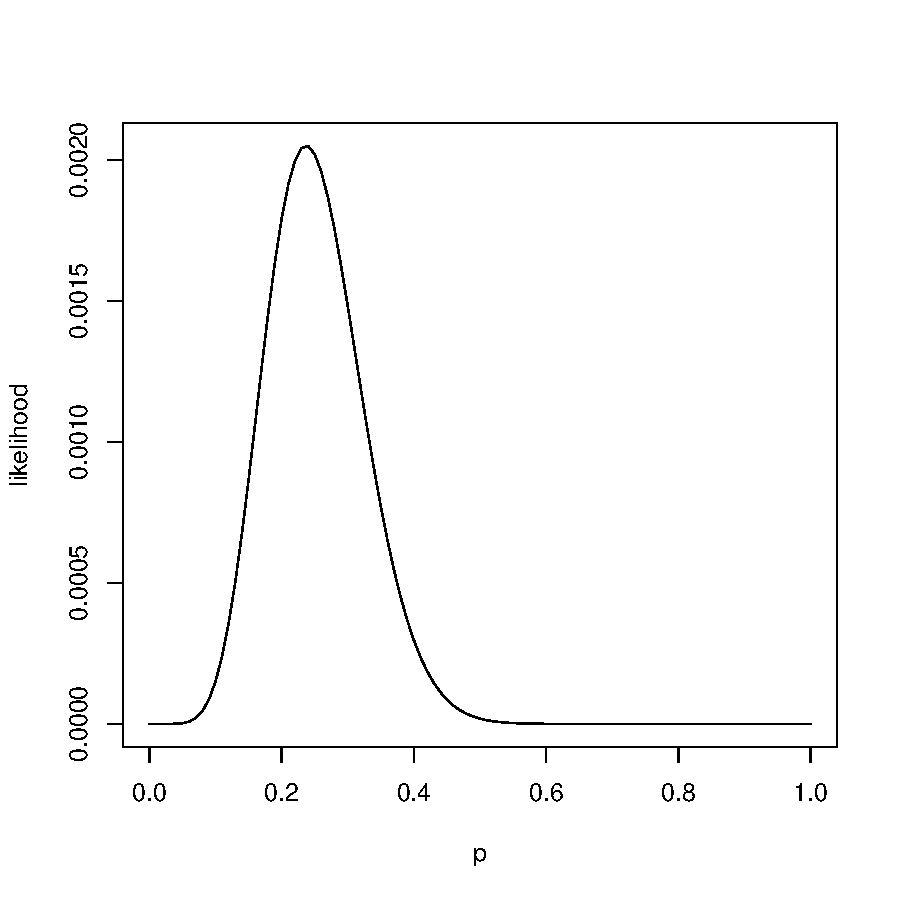
\includegraphics{chn_binom-006}

We can see the value of $p$ that maximizes the likelihood from the plot, but it's also very easy to ask R to tell us what it is explicitly:

\begin{Schunk}
\begin{Sinput}
> seq(0,1,0.01)[which(lvec==max(lvec))]
\end{Sinput}
\begin{Soutput}
[1] 0.24
\end{Soutput}
\end{Schunk}

\subsection*{$\mathcal{L} (p|x) \propto \text{prob}(x|p)$}
Provided the likelihood is proportional to $\text{prob} (x|p)$ we can proceed as above and find $p$ that maximizes likelihood. We can exploit the fact that the binomial coefficients only have the effect of acting as a scalar multiplier of the likeihood function, meaning that they can be neglected from the calculation of likelihood and still provide the same estimate of $p$:

\begin{Schunk}
\begin{Sinput}
> lvec<-NULL
> for (pp in seq(0,1,0.01)){
+ my.l<-1
+ for (j in 1:9){
+ f<-1-(1-pp)^results$i[j]
+ my.l<-my.l*f^(results$i[j+1])*(1-f)^(results$s[j+1])
+ }
+ lvec<-c(lvec,my.l)
+ }
> plot(seq(0,1,0.01),lvec,type="l",xlab="p",ylab="likelihood")
\end{Sinput}
\end{Schunk}
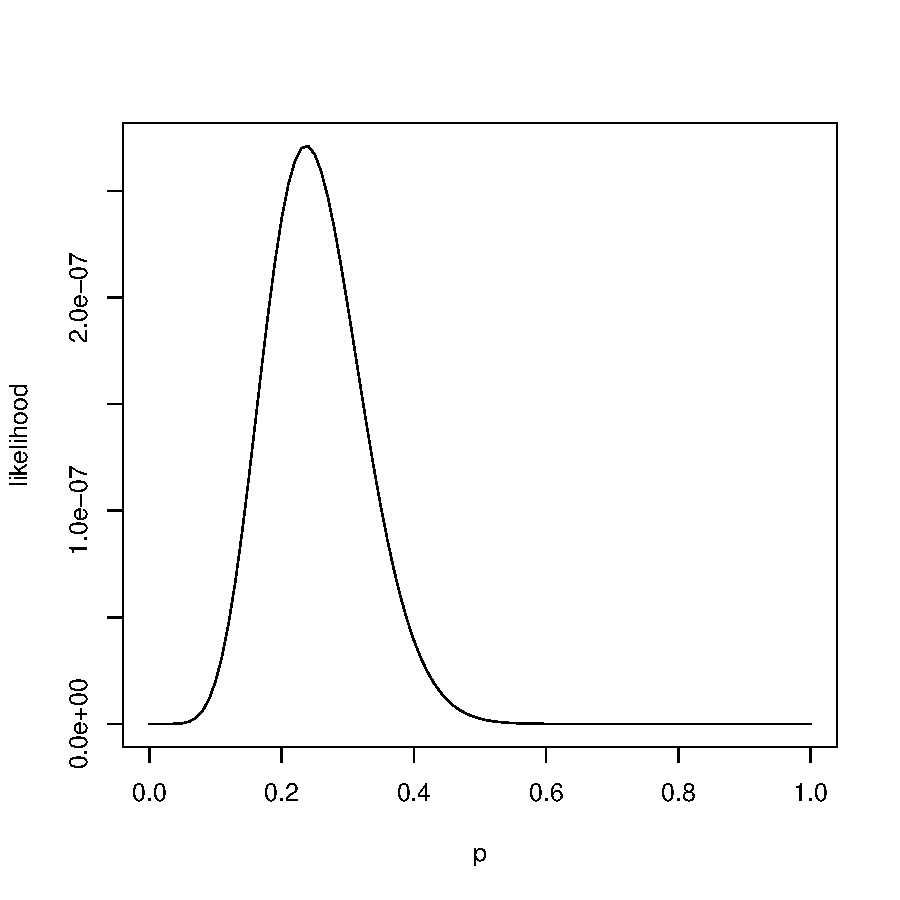
\includegraphics{chn_binom-008}

With this more efficient method, the estimate of $p$ should be the same as before:

\begin{Schunk}
\begin{Sinput}
> seq(0,1,0.01)[which(lvec==max(lvec))]
\end{Sinput}
\begin{Soutput}
[1] 0.24
\end{Soutput}
\end{Schunk}


\subsection*{Robustness of the estimate}
If we only had one data set, that would pretty much be the end of this study. Given that we simulated the data, we can change simulations or add them to get additional insight into robustness of the estimate and factors that make estimates more or less uncertain. First, let's simulate our small outbreak multiple times, each time recording the value of $p$ that maximizes the likelihood. 


\begin{Schunk}
\begin{Sinput}
> pvec<-NULL # a place to store all the maximum likelihood estimates
> for (rep in 1:1000){ # perform many versions of the outbreak from same initial conds/same p
+ # chain binomial model for outbreak
+ s.now<-9
+ i.now<-1
+ r.now<-0
+ # store time step and state variables in a dataframe called "results"
+ results<-as.data.frame(matrix(c(0,s.now,i.now,r.now),nrow=1))
+ # label column headings 
+ names(results)<-c("t","s","i","r")
+ # define transmission probability
+ my.p=0.3
+ # take 9 time steps forward in addition to the first time (where initial conditions apply)
+ for (j in 1:9){ 
+ # work out number of infections
+ i.next<-rbinom(1,s.now,(1-(1-my.p)^i.now))
+ # update states, now at next time point
+ r.now<-r.now+i.now
+ s.now<-s.now-i.next
+ i.now<-i.next
+ # write time step and state variables to results dataframe
+ results<-rbind(results,c(j,s.now,i.now,r.now))  
+ }
+ lvec<-NULL
+ for (pp in seq(0,1,0.01)){
+ my.l<-1
+ for (j in 1:9){
+ p<-1-(1-pp)^results$i[j]
+ my.l<-my.l*choose(results$s[j],results$i[j+1])*p^(results$i[j+1])*(1-p)^(results$s[j+1])
+ }
+ lvec<-c(lvec,my.l)
+ }
+ #plot(seq(0,1,0.01),lvec,type="l",xlab="p",ylab="likelihood")
+ pvec<-c(pvec,((which(lvec==max(lvec)))-1)/100)
+ }
> hist(pvec,breaks=50,main="true value shown in red",xlim=c(0,1))
> abline(v=my.p,col="red")
\end{Sinput}
\end{Schunk}
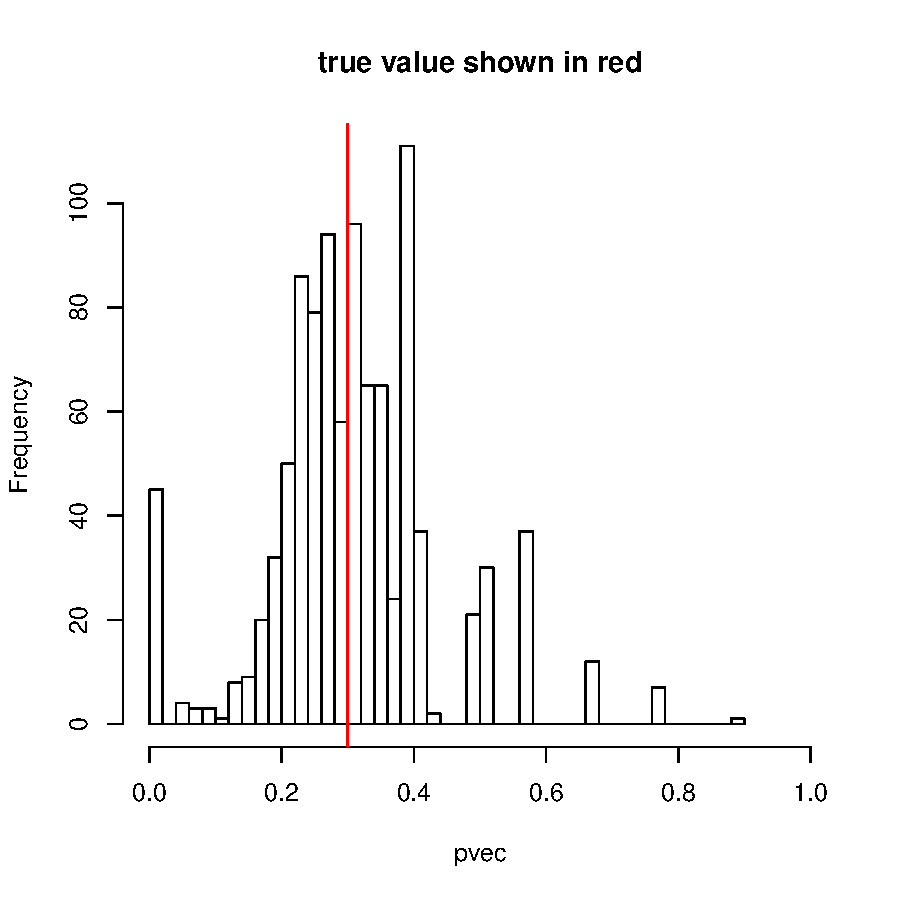
\includegraphics{chn_binom-010}

With a fixed population size of ten individuals (as we have) outbreak data is rather coarse. We could see if the estimation procedure performs better in bigger populations (in Sweave I've set echo=FALSE here so you won't see the code in the PDF but it is the same as above with the initial number of susceptibles (s.now) changed from 9 to 99):

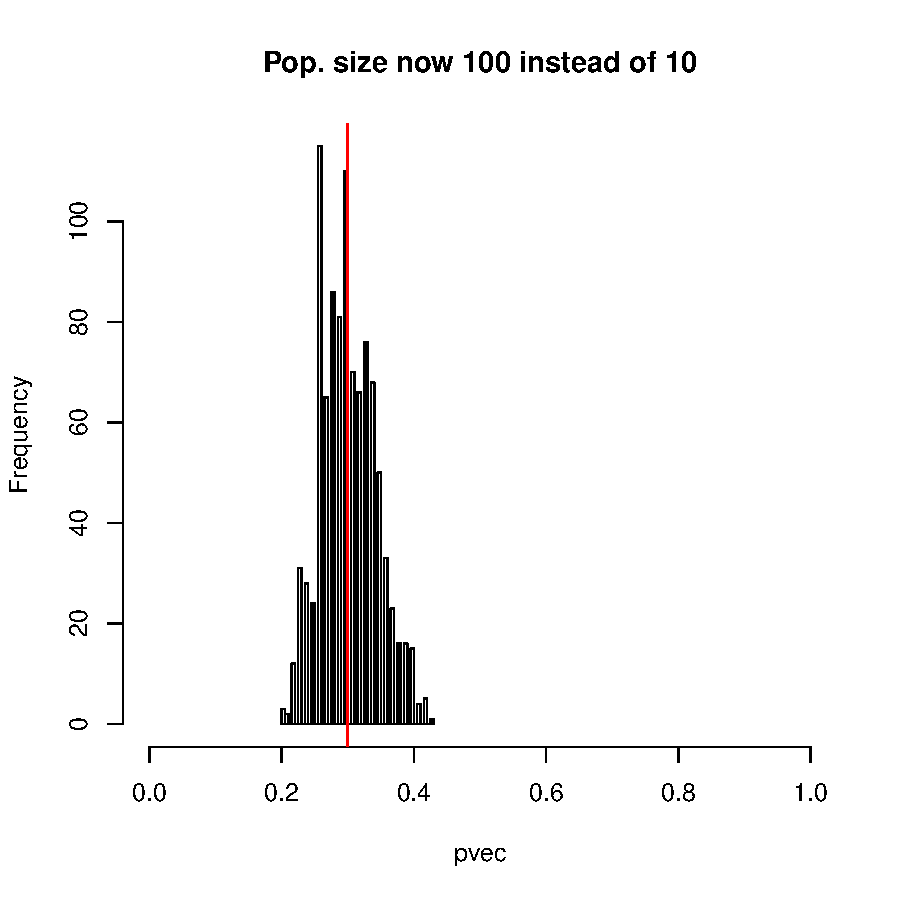
\includegraphics{chn_binom-011}

We may also be interested to know if the value of $p$ itself makes its estimation more or less difficult (i.e. whether $p$ represents an intermediate versus extreme probability).

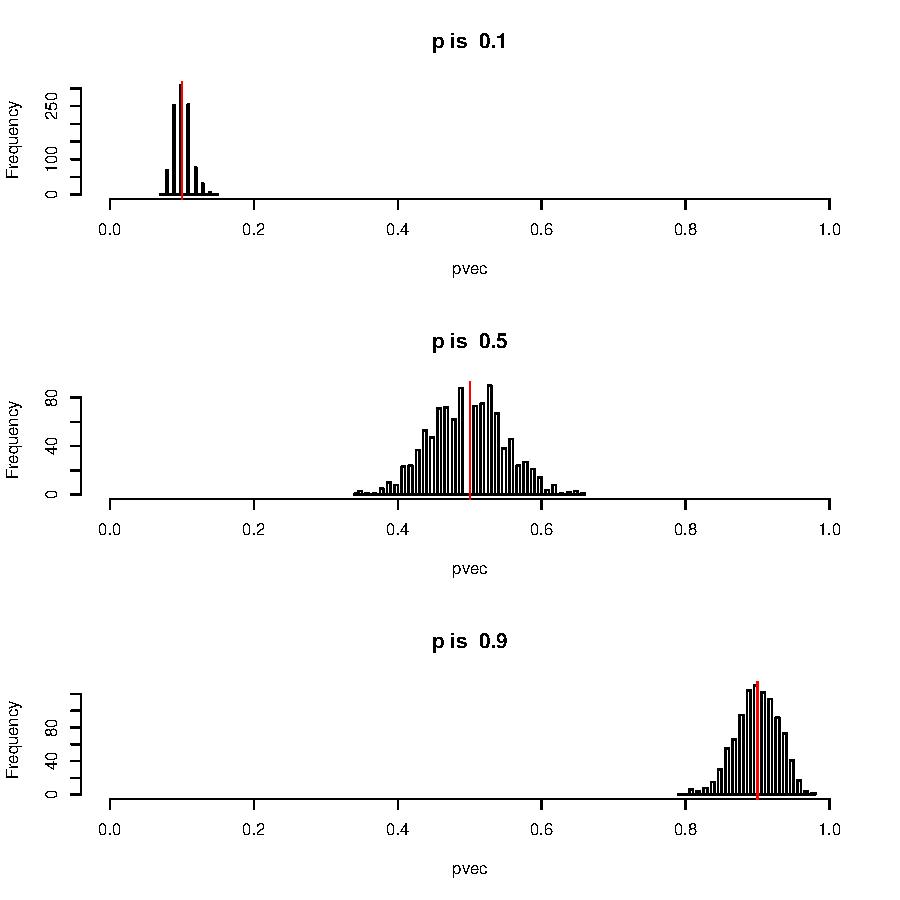
\includegraphics{chn_binom-012}

\section*{Negative log likelihood}
In practice (as reflected in the literature) it often makes sense to work with the negative log likelihood. The log transformation improves numerical accuracy (rounding errors) and numerical performance. Negating the log likelihood is simply done as many off-the-shelf optimizing routines are designed to minimize functions rather than mazimize them. Here we demonstrate the maximum likelihood technique with negative log likelihood and R's built in optimizing routine ``optim'':

\begin{Schunk}
\begin{Sinput}
> # chain binomial model for outbreak
> # initial conditions
> s.now<-9
> i.now<-1
> r.now<-0
> # store time step and state variables in a dataframe called "results"
> results<-as.data.frame(matrix(c(0,s.now,i.now,r.now),nrow=1))
> # label column headings 
> names(results)<-c("t","s","i","r")
> # define transmission probability
> p=0.3
> # take 9 time steps forward in addition to the first time (where initial conditions apply)
> for (j in 1:9){ 
+ # work out number of infections
+ i.next<-rbinom(1,s.now,(1-(1-p)^i.now))
+ # update states, now at next time point
+ r.now<-r.now+i.now
+ s.now<-s.now-i.next
+ i.now<-i.next
+ # write time step and state variables to results dataframe
+ results<-rbind(results,c(j,s.now,i.now,r.now))  
+ }
> p01<-0.5 # guess parameter
> # define the function to be optimized (needs data and parameters)
> my.nll<-function(p01,results){
+ z<-0
+ for (j in 2:9){
+ y<-(1-(1-p01)^results$i[j-1])
+ # adding log likelihoods is like multiplying likelihoods (here we subtract as we want to minimze)
+ z<-z-(log(y^results$i[j]*(1-y)^results$s[j]))
+ }
+ return(z)
+ }
> z2<-optim(par=p01,fn=my.nll,method="Brent",lower=0,upper=1,results=results)
> print(z2)
\end{Sinput}
\begin{Soutput}
$par
[1] 0.2848509

$value
[1] 13.48256

$counts
function gradient 
      NA       NA 

$convergence
[1] 0

$message
NULL
\end{Soutput}
\end{Schunk}

This technique also provides the value of $p$ that maximises likelihood (or equivalently, minimizes log likelihood):

\end{document}
